\documentclass{article}
\usepackage[utf8]{inputenc}
\usepackage{geometry}
\usepackage[export]{adjustbox}
\geometry{top=2cm, bottom=2cm, left=1.5cm, right=1.5cm}
\usepackage{titlesec}
\usepackage{lipsum}
\usepackage{fancyhdr}
\usepackage{enumitem}
\usepackage{hyperref}
\hypersetup{colorlinks=true,  linkcolor=black, citecolor=black, urlcolor=blue}
\hypersetup{pdfborder=0 0 0}
\usepackage{graphicx}
\usepackage{caption}
\usepackage{subcaption}

\usepackage[ngerman]{babel}
\usepackage{pythonhighlight}


\title{\textbf {Inwieweit nimmt Elon Musk durch sein Verhalten auf der Social Media Plattform X (ehem. Twitter) Einfluss auf den Kursverlauf von Tesla und Dogecoin?}}

\author{Eine Analyse und Bewertung der Big Data Bandits \\ (Daniel Linck, Daniel Weißenberger, David Helwich, Jonas Sigmund)}
\date{\today}

\begin{document}


\maketitle

\tableofcontents
\newpage

\section{Einleitung}
Da gerade das digitale Zeitalter geprägt von dem Einfluss großer Social-Media Plattformen ist, haben die Big Data Bandits beschlossen diese Extremen genauer zu betrachten.
Unter dem Aspekt, dass Elon Musk wohl zu den populärsten, einflussreichsten und dominantesten Personen des öffentlichen Lebens zählt, nominiert ihn insbesondere sein ``besonderes'' Korrespondenzverhalten gepaart mit seinen wirtschaftlichen Interessen für eine genauere Untersuchung.
Im folgenden Abstract findet eine Beantwortung und Beurteilung der Fragestellung im Ramen der gestellten Aufgabe statt.
Dafür analysieren wir die entsprechenden Datensätze mit einem für die Aufgabe entworfenem Python Script.
Dieses kann, aufgrund seiner hohen Modularität, auch in der Zukunft zur Beantwortung ähnlicher Fragestellungen verwendet werden.
Weitere Details bezüglich des Codes können der \href{https://github.com/alphaname007/BigDataBandits/blob/17e158a26d8d1cc538102ff44e4171b609965e95/code\_main.ipynb}{code\_main.ipynb} entnommen werden.



\section{Fragestellung}
Die Fragestellung: ``Inwieweit nimmt Elon Musk durch sein Verhalten auf der Social Media Plattform X (ehem. Twitter) Einfluss auf den Kursverlauf von Tesla und Dogecoin?'' wurde in mehreren Iterrationsschritten optimiert. 
Dies ist insbesondere dem Zeitraum geschuldet, in welchem die Auswertung abgeschlossen sein musste.
Somit war es uns zwar nicht möglich, eine allgemeinere Fragestellung über den allgemeinen Einfluss von Privatpersonen auf den Aktienmarkt unter der Berücksichtigung verschiedener Personen zu beantworten.
Jedoch konnten wir nun zusätzliche Legalitätsapekte, sowie konkrete Empfehlungen für ein profitables Investieren als Privatperson mit in unsere Ausarbeitung nehmen.



\section{Datensätze}
Die Datensätze entstammen der Community-Plattform \href{https://www.kaggle.com/datasets/dhruvildave/dogecoin-historical-data}{Kaggle}.
Im Folgenden verwenden wir einen Datensatz, der alle Posts (``Tweets'') des Tesla-CEOs Elon Musk  beinhaltet: \href{https://www.kaggle.com/datasets/aryansingh0909/elon-musk-tweets-updated-daily}{Posts}, sowie zwei weitere Datensätze, die den Kursverlauf von \href{https://www.kaggle.com/datasets/dhruvildave/dogecoin-historical-datay}{Dogecoin} und \href{https://www.kaggle.com/datasets/dhruvildave/dogecoin-historical-datay}{Tesla} umfassen.
Alle Datensätze vermitteln einen seriösen und schlüssigen Eindruck, was unter anderem an den fehlerfreien und plausiblen Werten liegt.
Zudem wurde der Tesla-Datensatz an den Aktiensplit angepasst und unter Verwendung der offiziellen Yahoo Finance API erstellt.
Für die Auswertung werden insbesondere die Zeilen ``date'' und ``raw\_close'' der Stock-Datensätze, sowie die Spalten ``datetime'' und ``text'' des Post-Datensatzes betrachtet.


\subsection{Data Understanding}

\subsubsection{Datendichte}
\begin{figure}[!htb]
  	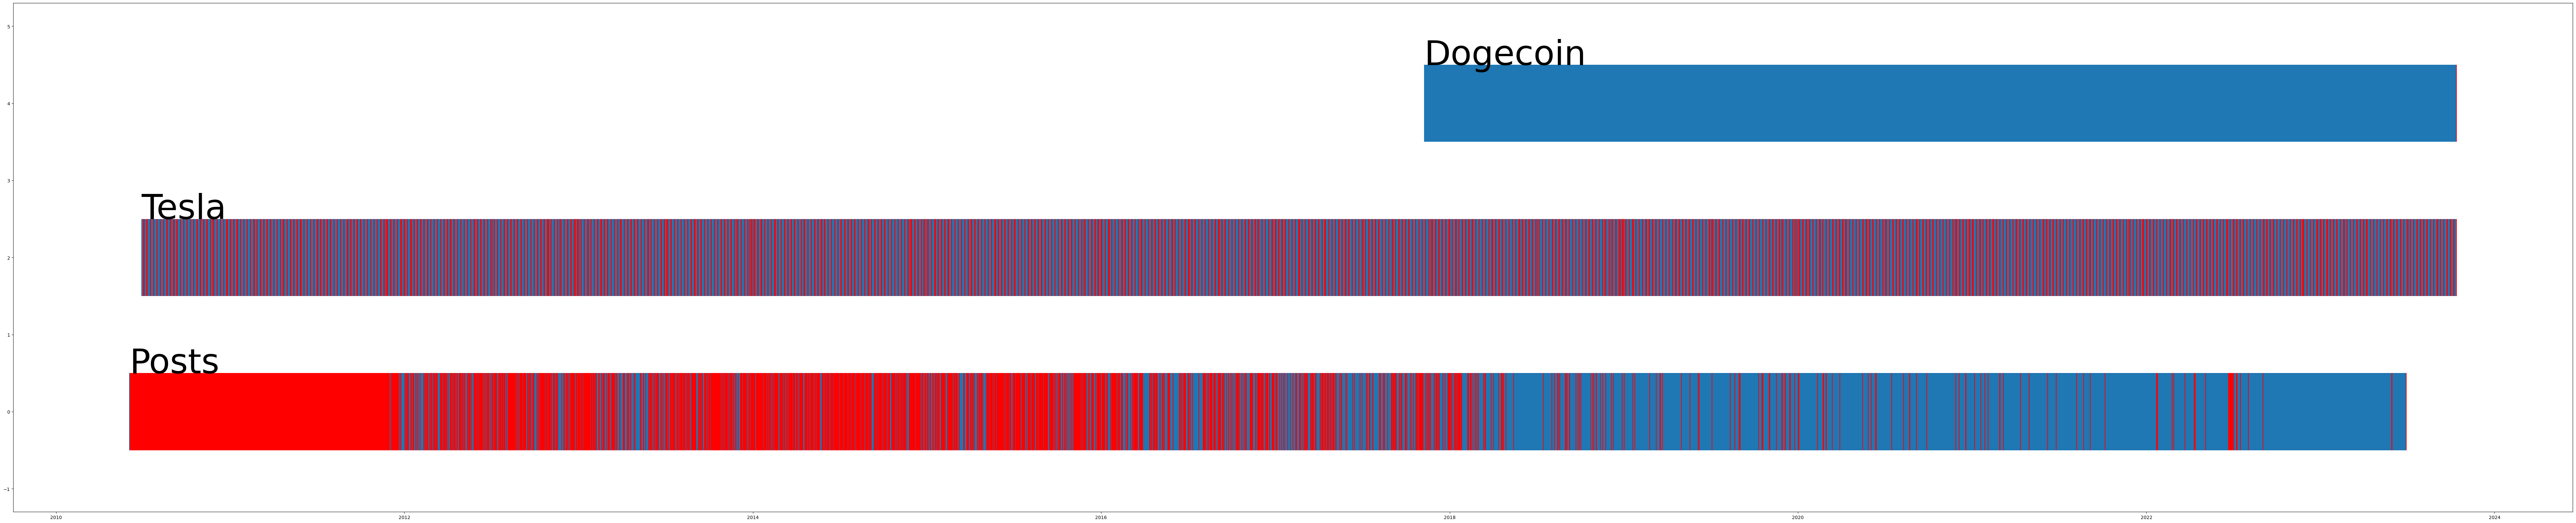
\includegraphics[width=.7\textwidth, height=100px]{../imgs/Dichte1.png}
	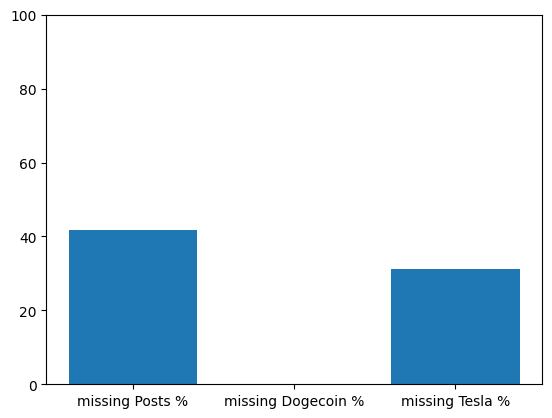
\includegraphics[width=.3\textwidth, height=100px]{../imgs/Dichte2.png}
 	\caption{Datendichte}
 	\label{fig:Datendichte}
\end{figure}
Die erste Grafik zeigt die gesamte Zeitspanne (04.06.2010 - 12.10.2023) aller gesammelter Daten aus den drei Datensätzen.
Dabei beschreibt der rote Anteil alle fehlenden Tage des jeweiligen Datensatzes.
Die Regelmäßigkeit der fehlenden Daten im Tesla-Datensatz kann auf die geschlossenen Tage der Aktienbörse zurückgeführt werden;
demzufolge, weist der Dogecoin-Datensatz auch keine fehlenden Datensätze auf, da die Kryptomärkte keiner Schließzeit unterliegen.
Die prozentuale Anzahl der fehlenden Tage kann der zweiten Grafik entnommen werden.
Darüber hinaus lässt sich aus dem Schaubild die Aussage ableiten, dass das Korrespondenzverhalten von Elon Musk auf der Plattform X über die Zeit zunimmt.
Zusammen mit der eineinhalbjährigen Pause nach seinem ersten Tweet am 04.06.2010 lässt dies die Vermutung offen, dass Musk erst nach und nach das Potenzial der Plattform erkannte, bis er diese schließlich am 04.04.2022 unter fragwürdigen Umständen aufkaufte. 
Die Auswertung der fehlenden Tage wird durch die Methode \textit{get\_density(df:pd.DataFrame)} ermöglicht, welche zunächst eine Liste aller Tage erstellt, die im jeweiligen Datensatz vorhanden sein sollten.
Im Folgenden wird ein neuer Datensatz erstellt, der alle Tage, sowie den entsprechenden booleschen Wert (1 vorhanden / 0 fehlend) für jeden Tag des zu untersuchenden Datensatzes enthält.
Dieser resultierende Datensatz kann nun einfach mit einem Eventplot skizziert werden und bietet die einfache Möglichkeit, den Prozentsatz der fehlenden Tage zu ermitteln.
\begin{python}
def get_density(df:pd.DataFrame):
    start_date = min(df["date"]).replace(hour=0, minute=0, second=0, microsecond=0)
    end_date = max(df["date"]).replace(hour=0, minute=0, second=0, microsecond=0) + pd.Timedelta(days=1)
    all_dates = pd.DataFrame({"date": pd.date_range(start_date, end_date, freq='D')})
    all_dates["exists"] = all_dates["date"].isin(df["date"]).astype(int)
    return all_dates
\end{python}


\subsection{Data Preperation}
Da die Datensätze schon sehr gut strukturiert sind, ist es nicht nötig eine erweiterte Datapreperation durchzuführen.
Optional könnten die ungenutzten Spalten entfernt werden, um Rechenzeit und Speichergröße zu verbessern, jedoch ist beides unerheblich und würde die Weiterentwicklung erheblich einschränken.



\section{Lösungsansatz}


\subsection{Hilfsfunktionen}

\subsubsection{Intervalselection}
Die Methode \textit{check\_filter()} erkennt, ob in einem Text gewisse Schlüsselwörter aus einer Filter-Liste enthalten sind.
Dies ermöglicht das Filtern der Posts anhand der evtl. im Post (Tweet) enthaltenen Schlüsselwörter (bsp.: ``Dogecoin'').
Dabei kann in abhängigkeit der Variable \textit{hit}, entwedern nach dem vorhandenen sein (hit=True) oder dem fehlen (hit=Flase) der Schlüsselwörter sortiert werden.
Die Methode \textit{get\_interval} generiert einen Datensatz-Ausschnitt, der ausgehend von einem Startdatum die nächsten vorhandenen n Tage aus einem Stock-Datensatz enthält.
Die Anzahl der Tage wird durch den Parameter \textit{interval\_length} gegeben und beträgt Standartmäßig den Wert 5 (eine Arbeitwoche).
Es wird auserdem berücksichtigt, dass das Startdatum nicht im Stock-Datensatz enthalten ist.
In diesem Fall nimmt das Unterprogramm das nächste vorhandene Datum.
Ausgehend von dem gefundenen Datum, werden der Start-Index sowie der End-Index des Datensatz-Ausschnittes berechnet.

\subsubsection{Kursverlauf}


\subsection{Hauptschleife}
Die Hauptfunktion umfasst die grundlegende Schleife zur Auswertung der Datensätze in Bezug auf die Fragestellung.
Dafür wird ein neuer Datensatz "influence" erstellt, der für jeden Tag, an dem ein Post mit den entsprechenden Filterkriterien verfasst wurde, das Datum, eine Liste aller Posts, die Anzahl dieser Posts sowie den prozentualen Unterschied der dafür vorgesehenen Hilfsfunktionen enthält.
So iteriert diese Schleife zunächst über alle Posts (Tweets), die im Datensatz Posts enthalten sind.
Im Anschluss wird nun durch die Methode check\_filter überprüft, ob die aktuelle Zeile den Filteransprüchen gerecht wird.
Trifft dies nicht zu, so wird diese Zeile übersprungen.
Ansonsten wird das Datum aus der aktuellen Zeile ausgelesen.
Im Folgenden wird nun überprüft, ob der aktuelle Tag schon im Datensatz ``influence'' enthalten ist, was passiert, wenn an einem Tag mehrere Posts vorliegen. Trifft dies zu, so wird dieser nur um den aktuellen Posttext ergänzt, sowie die Anzahl der Posts an diesem Tag inkrementiert.
Ist dieser Tag noch nicht im Datensatz influences enthalten, so wird für den aktuellen Tag zunächst das Intervall des Stock-Datensatzes bestimmt.
Ist dies nicht möglich, so wird eine Warnung ausgegeben und die Schleif fährt fort.
(Dies ist jedoch wie in 3.3.1 beschrieben zu vernachlässigen).
Wenn das Intervall erfolgreich erstellt wurde, werden nun alle Berechnungen auf das Intervall angewandt.
Schlussendlich werden nun alle Werte unter diesem Tag in den Datensatz ``influences'' eingefügt.
Hat die Schleife nun alle Posts abgearbeitet, kann nun dieser Datensatz zurückgegeben werden.
Zudem wird nun noch der prozentuale Anteil der im ``influence'' enthaltenen Posts von allen Posts ermittelt und zurückgegeben werden.
\begin{python}
def get_influence(stock:pd.DataFrame, posts:pd.DataFrame=Posts, filter_list:list=[], hit:bool=False,):
    # find a common start date
    start_date = max(posts['date'].min(), stock['date'].min())
    # adjust Posts to startdate
    posts = posts[posts['date'] >= start_date]
    # adjust Stock to startdate
    stock = stock[stock['date'] >= start_date]

    influence:pd.DataFrame = pd.DataFrame(columns=['date', 'posts', 'count_posts', 'trend', 'absolute'])
    j = 0
    old_date = None
    for i, post in posts.iterrows():
        if not check_filter(str(post['text']), filter_list, hit=hit):
            continue
        else:
            date = pd.to_datetime(post['date']).normalize()
            if not date == old_date:
                interval = get_interval(date, stock)
                if interval is None:
                    print("No Data Available")
                    continue
                cp_trend, model = get_trend(interval)
                cp_absolute = get_absolute(interval)
                influence.loc[j] = [date] + [[post['text']]] + [0] + [cp_trend] + [cp_absolute]
                old_date = date
                j += 1
            else:
                influence.loc[j-1, 'posts'].append(post['text'])
                influence.loc[j-1, 'count_posts'] += 1
    return [influence, j/i*100]
\end{python}

\subsection{Erzeugung}
Filter..


\newpage

\section{Auswertung}
\subsection{Posts}
\subsubsection{Verteilung}
\begin{figure}[h]
  	\centering
  	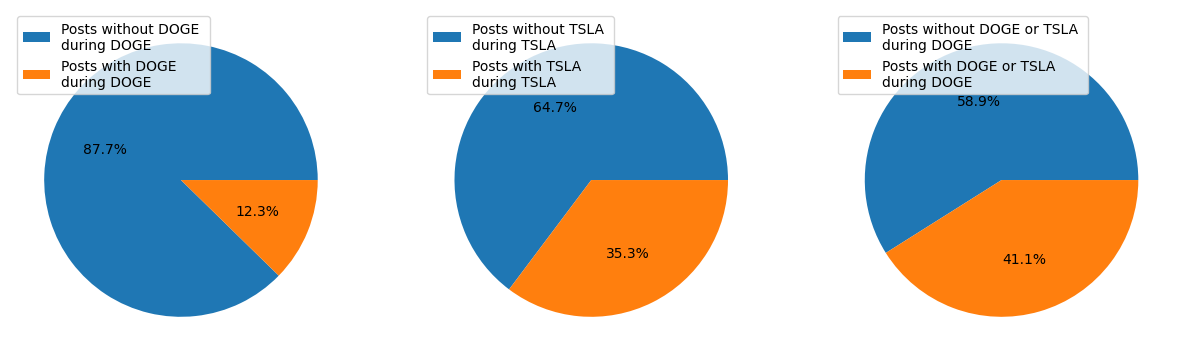
\includegraphics[width=\textwidth]{../imgs/Verteilung.png}
 	\caption{Verteilung}
 	\label{fig:Verteilung}
\end{figure}
Dieses Diagramm zeigt die Verteilung der entsprechenden Schlüsselwörter in allen Posts des zu betrachtenden Zeitraums.
Dabei ist es wichtig zu beachten, dass der zu betrachtende Zeitraum zusammen mit den Aufzeichnungen des Kursverlaufs beginnt.
Demzufolge wird beispielsweise die Verteilung der Schlüsselwörter für Dogecoin nur für den Zeitraum des Dogecoin-Datensatzes erstellt.
Interessant ist hierbei insbesondere die Tatsache, dass Elon Musk fast doppelt so viel über Tesla ``twittert'' als über Dogecoin.
Insbesondere wenn man sich die kombinierten Schlüsselwörter über den Zeitraum des Dogecoin-Datensatzes (da Dogecoin-Datensatz \textless Tesla-Datensatz) (3. Kuchendiagramm) näher anschaut, ist deutlich zu erkennen, dass selbst hier Tesla einen Anteil von 28.8\% besitzt (da 41.1\%-12.3\%).
Dies ist immer noch mehr als doppelt so viel als die 12.3\% der Dogecoin-Posts.
Dies könnte daran liegen, dass Dogecoin von Elon Musk mehr als eine Art Neben- oder Spaßprojekt angesehen wird; seine Verbundenheit zu Tesla ist wohl auch schon alleine durch seine Position (CEO) gegeben.

\subsubsection{Verlauf}
\begin{figure}[!htb]
  	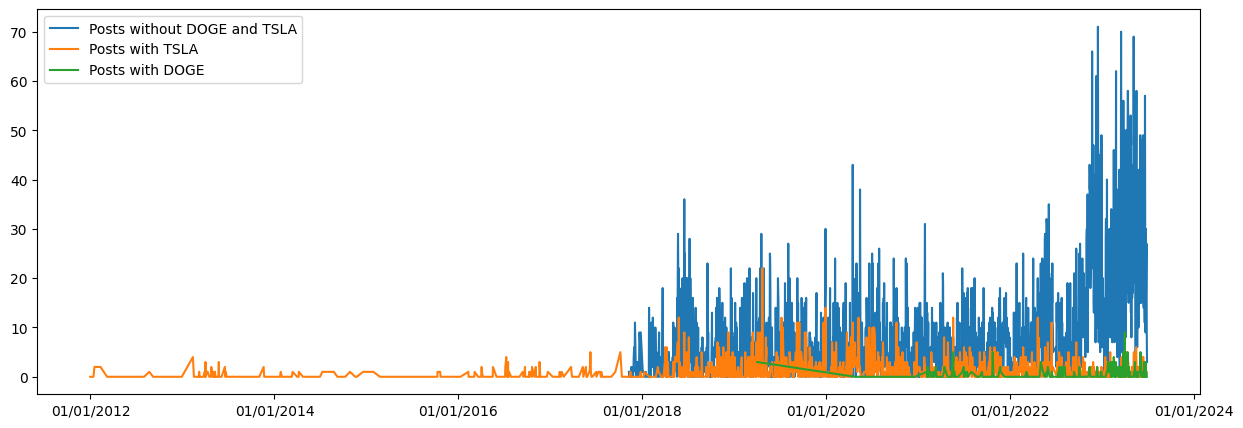
\includegraphics[width=\textwidth, center]{../imgs/Verlauf.png}
 	\caption{Datendichte}
 	\label{fig:Datendichte}
\end{figure}
Dieses Diagramm zeigt den Tag (x-Achse), sowie die Anzahl der Posts an diesem Tag (y-Achse). Auch hier sieht man die in \ref{sec:Dataunderstanding} aufgeworfene These, das das Korrespondenzverhalten von Elon Musk im Verlauf der Zeit zunimmt.
Zudem wird diese Vermutung nun auch durch die Anzahl der Posts an einem Tag gestützt.
Denn dieser ist zu entnehmen, dass Elon Musk nicht nur an mehreren Tagen, sondern vor allem auch deutlich häufiger pro Tag ``Tweeted''.
Dieses Verhalten kann insbesondere seit der Übernahme der Plattform am 04.04.2022 beobachtet werden.
Während im Sommer 2019 ein Großteil seiner Posts die Schlüsselwörter von Tesla beinhalteten, postet Elon Musk mittlerweile schon fast genau so viel über Dogecoin wie über Tesla. Das könnte ein Indiz dafür sein, dass Dogecoin für Musk zurzeit an Interesse gewonnen hat.

\subsubsection{Zusammenhänge}
\begin{figure}[!htb]
	\begin{minipage}{0.4\textwidth}
    		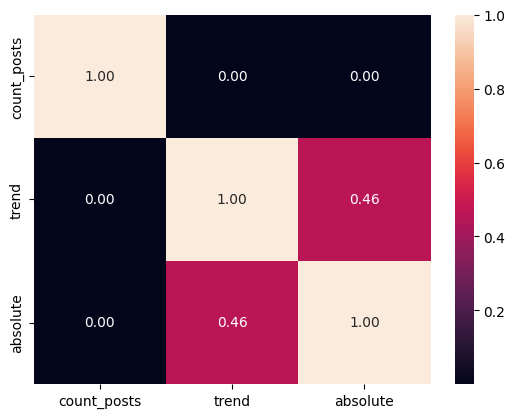
\includegraphics[width=\textwidth]{../imgs/Korrelation.png}
    		\caption{Korrelation}
    		\label{fig:Korrelation}
  	\end{minipage}
  	\hfill
	\begin{minipage}{0.55\textwidth}
		Der wichtigste Aspekt, der der Korrelationstabelle des Einfluss-Datensatzes entnommen werden kann, ist die Unabhängigkeit zwischen der Spalte ``count\_posts'' und den Werten ``trend'' und ``absolute''.
		Dies zeigt, dass die Anzahl der Posts (Tweets) an einem Tag keinen Einfluss auf den Verlauf der beiden Wertpapiere hat.
		Die Korrelationstabelle wurde unter Verwendung der Bibliothek Seaborn aus der Vereinigung der Schlüsselwort freien Einfluss-Datensätz erstellt.
	\begin{python}
	influences_corr = pd.concat(
	    [
	        influences_t_d[['count_posts', 'trend', 'absolute']],
	        influences_t_t[['count_posts', 'trend', 'absolute']]
	    ]
	).corr()
	sns.heatmap(influences_corr, annot=True, fmt=".2f")
	plt.show()
	\end{python}
		
	\end{minipage}
\end{figure}

\newpage



\subsection{Trend}
\subsubsection{Verlauf}
\begin{figure}[!htb]
  	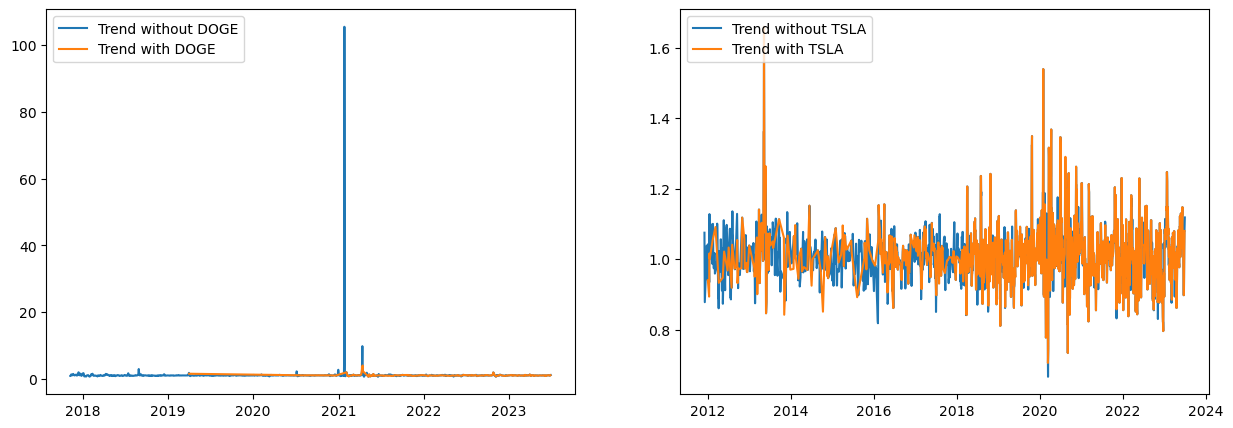
\includegraphics[width=\textwidth, center]{../imgs/Trend.png}
 	\caption{Trend}
 	\label{fig:Trend}
\end{figure}
Bei diesen Diagrammen wird jeweils der Trend von Doge und Tesla nach einem Post von Musk gezeigt. Einmal den Trend, wenn Musk einen Tweet mit Doge oder eben Tesla machte und einmal wenn er einfach nur einen Tweet machte, aber ohne Doge oder Tesla. Bei Doge erkennt man, dass der Trend kaum von Musks Tweets beeinflusst wird, da die Veränderung in \% immer recht gering/gleich ist, im Vergleich zu den Veränderungen ohne das
Schlüsselwort Doge, und manchmal sogar die Veränderung des Trends ohne Musks Tweets deutlich höher ist als mit. Bei Tesla haben Musks Tweets deutlich mehr Einfluss auf die Aktie, man kann deutlich erkennen das ab 2018 Musk mehr tweetete, aber auch das es einige Peeks gibt bei denen ein Tweet den Trend positiv, aber auch negativ veränderte. Mann sieht aber auch, dass die meiste Zeit der Trend ohne einen solchen Tweet ähnlich verläuft wie der Trend mit einem solchen Tweet. Daher kann man schließen, dass Musk durch seine Tweets zwar die Tesla Aktie beeinflussen kann, aber die Aktie auch immer noch von anderen (uns unbekannten) Faktoren abhängt. Meistens verhält sich die Aktie so, als würde Musk nicht den Markt beeinflussen, aber an manchen Punkten schafft er es schon den Trend der Aktie stark in eine Richtung zu lenken, dabei wissen wir jedoch nicht, ob er die Veränderung geplant hat oder es einfach zufällig geschah.

\subsubsection{Durchschnitt}
\begin{figure}[!htb]
  	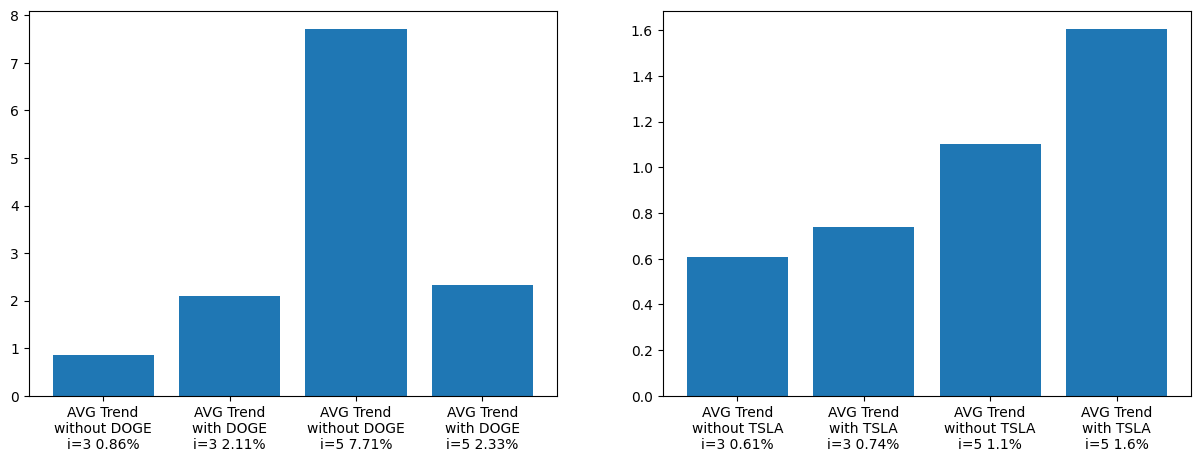
\includegraphics[width=\textwidth, center]{../imgs/Trend_Durchschnitt.png}
 	\caption{Trend Durchschnitt}
 	\label{fig:Trend Durchschnitt}
\end{figure}
In diesen Grafiken werden Tesla und Dogecoin anhand der Aktientrends verglichen. In beiden Fällen wird einmal der Trend genommen ohne, dass Elon Musk das Wort „TSLA“ oder „DOGE“ in seinen Tweets genutzt hat und einmal, wenn er es benutzt hat.
In der linken Grafik wird auf die Dogecoin Aktie geschaut, bei Tweets ohne die Verwendung des Wortes „DOGE“ und mit der Verwendung des Wortes „DOGE“ hier kann man gut sehen, dass der Trend ohne die Verwendung bei 1.08 liegt und mit der Verwendung bei 1.02.
Daraus kann man hier ziehen, dass Elon Musk durch die Verwendung des Wortes „DOGE“ in seinen Tweets einen Einfluss auf den Trend der Aktie Dogecoin haben kann. In diesem Fall aber sogar negativen Einfluss.
In der rechten Grafik wird auf die Tesla Aktie geschaut, hier wird nach Verwendung des Wortes "TSLA“ in seinen Tweets geschaut. Hier liegt der Wert ohne die Verwendung des Wortes bei 1.01 und wenn er es verwendet bei 1.02.
Dadurch kann man bei der rechten Grafik ziehen, dass es bei der Tesla Aktie keine wirklichen Auswirkungen auf den allgemeinen Trend der Aktie gab.


\subsection{Absolute}
\subsubsection{Verlauf}
\begin{figure}[!htb]
  	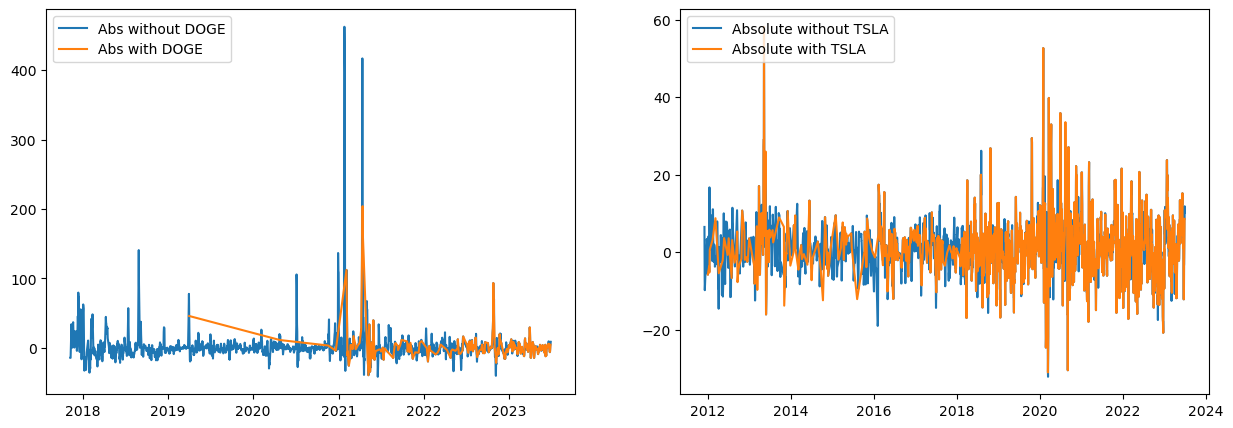
\includegraphics[width=\textwidth, center]{../imgs/Absolut.png}
 	\caption{Absolut}
 	\label{fig:Absolut}
\end{figure}
Nun haben wir die Absoluten werte in \% von Dogecoin und Tesla nach eine Post von Musk. Bei dem ersten Diagramm erkennt man, dass die Tweets über Dogecoin sogar weniger Einfluss haben als, wenn Musk einfach nur so twitterte, daraus lässt sich schließen, dass bei Dogecoin, Musks Einfluss so gering ist, dass er praktisch gar nicht vorhanden ist, oder zumindest irrelevant ist. Bei Tesla jedoch gibt es einige Punkte bei denen sich die Aktie stark veränderte, aufgrund bzw. nach einem Tweet von Musk. Jedoch sieht man auch das die Aktie auch ohne einen solchen Tweet sich oft stark veränderte, und somit kann man sagen das Musk zwar einen gewissen Einfluss hat, aber diesen nicht oft nutzt. Das könnte z. B. daran liegen, dass es eventuell illegal ist, oder die Menschen sonst erkennen würden, wann er manipuliert und das dann für sich ausnutzen würden.


\subsubsection{Durchschnitt}
\begin{figure}[!htb]
  	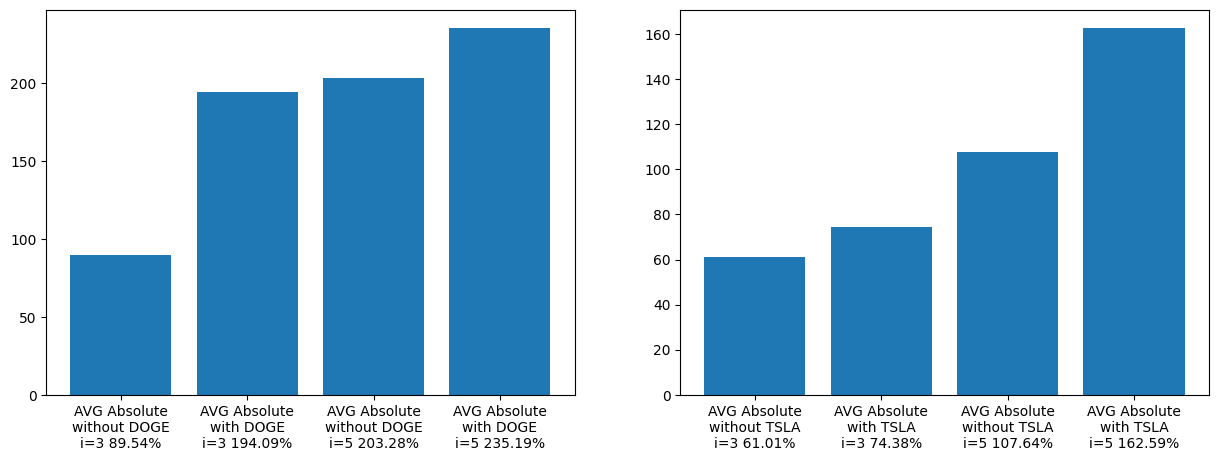
\includegraphics[width=\textwidth, center]{../imgs/Absolut_Durchschnitt.png}
 	\caption{Absolut Durchschnitt}
 	\label{fig:Absolut Durchschnitt}
\end{figure}
In dieser Grafik schauen wir uns die Auswirkung auf die absoluten Werte der beiden Aktien an, hier kann man direkt auf den ersten Blick einen etwas größeren Unterschied erkennen.
Bei ``DOGE'' ist der absolute Wert bei 2.03, wenn Elon Musk das Wort nicht in seinen Tweets genutzt hat, aber wenn er es benutzt hat, steigt der absolute Wert auf 2.35. Hieraus lässt sich schließen, dass er mit Sicherheit etwas Einfluss darauf hat, auch wenn es nicht viel ist.
Genau dasselbe mit der ``TSLA'' Aktie. Hier ist der absolute Wert bei 1.08, wenn er es in seinen Tweets nicht erwähnt, aber wenn es erwähnt wird, steigt der absolute Wert auf 1.63 an. Hier ist sein Einfluss sogar noch etwas stärker als bei DOGE.




\section{Gesamtbewertung / Erwartung}

\subsection{Die Legalität}
Die Legalität und die Auswirkung von Elon Musks Tweets auf den Aktienmarkt sind ein kompliziertes
Thema. Normalerweise müssen Äußerungen insbesondere von einflussreichen Personen, Managern
und Geschäftsführern von börsenorientierten Unternehmen in dem Rahmen der geltenden Gesetze
und Vorschriften erfolgen.
Die SEC (Securities and Exchange Commission) hat spezifische Regeln für Offenlegungen durch
Direktoren börsennotierter Unternehmen. Der Zweck dieser Regeln besteht darin, sicherzustellen,
dass relevante Informationen fair und gleichzeitig für alle Marktteilnehmer zugänglich sind. Musk und
Tesla standen in der Vergangenheit unter Beobachtung der SEC, insbesondere aufgrund von Elon
Musks Tweets über Tesla. Einige von Musks Tweets wurden als potenzielle Verstöße gegen die SEC-Regeln angesehen, was zu Rechtsstreitigkeiten und Vergleichen mit der SEC führte. Es ist wichtig zu beachten, dass die Rechtslage in solchen Fällen weitgehend von den konkreten Umständen und den
geltenden Gesetzen abhängt. Musk und sein Unternehmen müssen sich noch mit der öffentlichen
Kommunikation und ihren Auswirkungen auf den Aktienmarkt befassen.

\section{Fazit}

\end{document}
